\documentclass[tikz,border=5pt]{standalone}
\usepackage{tikz}
\begin{document}

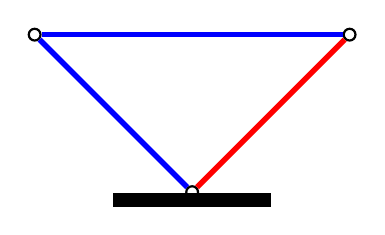
\begin{tikzpicture}[thick]
    % Nodes
    \node[draw, circle, fill=white, inner sep=1.5pt] (a) at (0,2) {};
    \node[draw, circle, fill=white, inner sep=1.5pt] (b) at (4,2) {};
    \node[draw, circle, fill=white, inner sep=1.5pt] (c) at (2,0) {};
    
    % Edges
    \draw[blue, line width=2pt] (a) -- (b);
    \draw[blue, line width=2pt] (a) -- (c);
    \draw[red, line width=2pt] (b) -- (c);
    \draw[black, line width=5pt] (1,-0.1) -- (3,-0.1);
    
\end{tikzpicture}

\end{document}